\part{Background}
\chapter{Electronic Structure Methods} % Main chapter title

\label{chap:meth}

NB: The notation in this chapter is largely borrowed from the following texts: \textit{Modern Quantum Chemistry: Introduction to Advanced Electronic Structure Theory} by Szabo and Ostlund,\cite{Szabo} \textit{Time-Dependent Density-Functional Theory: Concepts and Applications} by Ullrich,\cite{Ullrich} and \textit{Quantum Theory of the Solid State: An Introduction} by Kantorovich.\cite{Kantorovich2004}


\section{Wavefunctions Methods}

The state function of a nonrelativistic quantum mechanical system is wholly described by the Shr\"{o}dinger equation (SE):
\begin{equation}
    i\hbar \frac{d}{dt} \ket{\Psi(t)} = \hat{H} \ket{\Psi(t)}
    \label{eq:tdse}
\end{equation}
Where the $\ket{\Psi(t)}$ is the time dependent wave function, and $\hat{H}$ is the Hamiltonian operator. In a system of $N$ electrons and $M$ nuclei, $\hat{H}$ has the form:

\begin{equation}
    \hat{H} = - \sum_{i=1}^N \frac{1}{2} \nabla^2_i
              - \sum_{A=1}^M \frac{1}{2M_A} \nabla^2_A
              - \sum_{i=1}^N \sum_{A=1}^M \frac{Z_A}{r_{iA}}
              + \sum_{i=1}^N \sum_{j>i}^N \frac{1}{r_{ij}}
              + \sum_{A=1}^M \sum_{B>A}^M \frac{Z_AZ_B}{r_{AB}}
    \label{eq:full_hamilton}
\end{equation}

Where $\nabla^2_i$ and $\nabla^2_A$ are the Laplacian operators acting on electrons and nuclei respectively, $Z_A$ is the charge of nucleus $A$ and $r_{AB}$ is the distance between points $A$ and $B$.

In an equilibrium, the quantum system becomes time independent by definition, and has a simpler equation of state, the  time-independent Shr\"{o}dinger equation (TISE):\cite{Schrodinger1926}
\begin{equation}
    \hat{H} \ket{\Psi} =  E \ket{\Psi}
    \label{eq:tise}
\end{equation}
Where $\ket{\Psi}$ is the time independent wave function and $E$ its associated energy.

\subsection{The Born-Oppenheimer Approximation}

The SE is analytically unsolvable for any system with more than two particles. We must therefore employ approximations to model chemically meaningful situations.

Nuclei are several orders of magnitude heavier than electrons, suggesting that the Hamiltonian can be split into an electronic and a nuclear term. The electronic term treats nuclei as static potentials, and can yield an electronic wavefunction, uncorrelated with the nuclear one, which does not take into account the nuclear kinetic and internuclear potential terms of Equation \ref{eq:full_hamilton}:

\begin{equation}
    \hat{H}_{el} = - \sum_{i=1}^N \frac{1}{2} \nabla^2_i
              - \sum_{i=1}^N \sum_{A=1}^M \frac{Z_A}{r_{iA}}
              + \sum_{i=1}^N \sum_{j>i}^N \frac{1}{r_{ij}}
    \label{eq:el_ham}
\end{equation}

\begin{equation}
    \hat{H}_{el} \Phi = E_{el} \Phi
    \label{eq:el_tise}
\end{equation}

This is known as the Born-Oppenheimer (BO) approximation, and allows for the nuclear coordinates to be considered only parametrically when calculating the energy of a given nuclear geometry.\cite{Born1927}

\subsection{Many-Electron Wavefunctions}

Electrons are fermions of spin 1/2. Therefore the wavefunction which describes an electron should contain both a spatial part ($\psi(\bm{r})$), and a spin part ($\alpha(\omega)$ or $\beta(\omega)$ for spin up or down). Single electron wavefunctions are therefore called spin orbitals and, for example for spin up, are written:
\begin{equation}
\begin{split}
    \chi(\bm{x}) &= \psi(\bm{r})\alpha(\omega)\\
    \ket{\chi} &= \ket{\psi}\ket{\alpha}
    \label{eq:spinorb}
\end{split}
\end{equation}
Where the $\bm{x}$ coordinate contains both the position $\bm{r}$ and the spin $\omega$.

A many electron wavefunction should be constructed taking into account the properties of fermions that they are antisymmetric under exchange. To fulfil $\Psi(\bm{x_1},\bm{x_2}) = - \Psi(\bm{x_2},\bm{x_1})$, we can exploit the property of the matrix determinant, which changes sign with the interchange of row or column. This kind of wavefunction is called the Slater determinant:\cite{Slater1929}

\begin{gather}
    \Psi^{SD}(\bm{x_1},\bm{x_2},\ldots,\bm{x_N}) 
    = (N!)^{-1/2}
      \begin{vmatrix}
   \chi_i(\bm{x}_1) & \chi_j(\bm{x}_1) & \dotsm & \chi_k(\bm{x}_1) \\
   \chi_i(\bm{x}_2) & \chi_j(\bm{x}_2) & \dotsm & \chi_k(\bm{x}_2) \\
   \vdots           & \vdots           &        & \vdots           \\
   \chi_i(\bm{x}_N) & \chi_j(\bm{x}_N) & \dotsm & \chi_k(\bm{x}_N) 
   \end{vmatrix}
\end{gather}

In Dirac notation, we adopt the convention $\Psi^{SD}(\bm{x_1},\bm{x_2},\ldots,\bm{x_N}) = \ket{\bm{x_1}\bm{x_2}\ldots\bm{x_N}}$.


\subsection{The Hartree-Fock Method}
We now wish to find a method to compute all spin orbitals of the electronic system's Slater determinant to obtain the most accurate wavefunction possible. To do so, for each spin orbital, we write a one-electron secular equation:
\begin{equation}
    f(1)\chi(\bm{x}_1) = \epsilon  \chi(\bm{x}_1)
    \label{eq:one_electron_HF}
\end{equation}
    
$f(1)$ is called the Fock operator, and is written:

\begin{equation}
    f(1) = h(1) + v^{HF}(1)
\end{equation}{}

Where $h(1)$ is the one-electron core Hamiltonian:

\begin{equation}
    h(1) = - \frac{1}{2} \nabla^2_1 - \sum_{A=1}^M \frac{Z_A}{r_{1A}}
\end{equation}{}

And $v^{HF}(1)$ is the Hartree-Fock (HF) potential, associated with the multi-electronic interaction energy. It, in turn, is comprised of Coulomb and exchange electron-electron interactions, and is expressed:
\begin{equation}
    v^{HF}(1)=\sum_{b}(\mathcal{J}_b(1) - \mathcal{K}_b(1))
\end{equation}

Where the Coulomb operator $\mathcal{J}_b(1)$ expresses the electrostatic potential on the electron $1$ in orbital $\chi_a$ from electron $2$ in orbital $\chi_b$:
\begin{equation}
    \mathcal{J}_b(1) = \int \frac{|\chi_b(2)|^2}{r_{12}} d\bm{x}_2
\end{equation}
The exchange operator, on the other hand, is a nonlocal operator; it depends on the value of $\chi_a$ at points of space different from $\bm{x}_1$ as follows:
\begin{equation}
    \mathcal{K}_b(1)\chi_a(1) = \left[\int \chi_b(2)^*r^{-1}_{ij}\chi_a(2) d\bm{x}_2\right]\chi_b(1)
\end{equation}

In its full form, the Fock operator is therefore:\cite{Hartree1935,Fock1930,Fock1930a}

\begin{equation}
    f(1) = - \frac{1}{2} \nabla^2_1 - \sum_{A=1}^M \frac{Z_A}{r_{1A}} + \sum_{b} (\mathcal{J}_b(1) - \mathcal{K}_b(1))
\end{equation}

% In a closed shell system of $N$ electrons, the spatial Fock operator can be shown to adopt the form:
% \begin{equation}
%     f(1) = h(1) + \sum_a^{N/2} 2J_a(1)-K_a(1)
% \end{equation}
% where the closed-shell Coulomb and exchange operators are:
% \begin{equation}
%     \begin{split}
%         &J_a(1)=\int\psi^*_a(2)r^{-1}_{12}\psi_a(2)\\
%         &K_a(1)\psi_i(1) = \left[\int  \psi^*_a(2)r^{-1}_{12} \psi_a(1) d\bm{r}_2  \right] \psi_a(1)
%     \end{split}
% \end{equation}

\subsection{Atomic Orbital Basis Sets}
The two above operators involve the integration of products of spatial orbitals. If we could decompose these orbitals in an infinite number of functions spanning all of space, this would yield an exact spin orbital within the constraints of Hartree-Fock theory. However, due to the computational constraints of our finite central processing units, we must settle for an easily integrable set of functions which are arranged in a physically meaningful way. 

In the context of a molecular system, it makes most sense to employ sets of atom-centred functions which have the shapes of individual electrons about a particular nucleus. These are called atomic orbitals, and their linear combination makes up a molecular orbital. If our set has $K$ basis functions, we write spatial orbital $\psi_i$:

\begin{equation}
    \psi_{i} = \sum_{\mu = i}^K C_{\mu i}\phi_{\mu}
    \label{eq:lcao}
\end{equation}

For ease of integration, we often use a solutions of the hydrogen atom multiplied by Gaussian radial component. This is called a Gaussian Type Orbital (GTO). However, the behaviour of Gaussian functions in the limit of large distance does not necessarily reflect the behaviour of atomic orbitals, which instead follow an inverse law, thus in practice we use linear combinations of several GTOs, whose coefficients are called contractions, explaining the name Contracted Gaussian Functions (CGFs).

Oftentimes, the valence electrons are assigned more than one CGF, to obtain a better resolution of the interatomic interactions. Basis sets with several CGFs per valence electron are called split valence, or Pople basis sets if they are written in the form \textit{X-YZG}. For example, the basis set 6-31G has six GTOs per core electron basis function, and two CFGs for valence electrons, one with three GTOs and one with one GTO.

Additionally, the basis sets may be complemented by diffuse Gaussians to accurately describe the region of the atom far from the nucleus, or asymmetric functions to represent the polarisability of the atom. A 6-31G basis set complemented by diffuse and polarisable functions is written 6-31G(d,p).

\subsection{The Roothaan Equations}

Armed with our basis set, we are able to re-write the HF equation in matrix form by enclosing the Fock operator with basis functions. We write:

\begin{equation}
    \bm{F} \bm{C} = \bm{S} \bm{C} \bm{\epsilon}    
\label{eq:rooth}
\end{equation}

Where the Fock matrix has elements $F_{\mu \nu} = \int \phi^*_{\mu}(1)f(1)\phi_{\nu}(1)d\bm{r}_1$, $\bm{S}$ is the overlap matrix with elements $S_{\mu \nu} = \int \phi_{\mu}^*(1) \phi_{\nu}(1) d\bm{r}_1$, which account for the nonorthogonality of the basis, $\bm{C}$ defines the basis coefficients of the spin orbitals in Equation \ref{eq:lcao}, and $\bm{\epsilon}$ is the diagonal matrix of orbital energies:

\begin{gather}
    \bm{\epsilon} =
  \begin{pmatrix}
    \epsilon_{1} & & \mbox{\Large 0}\\
    & \ddots & \\
    \mbox{\Large 0} & & \epsilon_K
  \end{pmatrix}
\end{gather}

 The equations originating from the canonical Equation \ref{eq:rooth} are called the Roothaan equations. They can be manipulated to become orthogonal, and adopt a solvable form without the interfering overlap matrix. A particularity of the Roothaan equations is that since the Fock matrix contains the HF potential, it depends on the spin orbitals, which are themselves defined in $\bm{C}$. This indicates that the Roothaan equations must be solved iteratively, in order to find a self-consistent set of spin-orbitals. This procedure is known as the Self-Consistent Field (SCF) method.

The SCF method allows us to obtain a set of $K$ spatial orbitals and thus $2K$ spin orbitals. If we construct a wavefunction which is the Slater determinant of the $N$ lowest spin orbitals, we obtain the HF ground state:
\begin{equation}
    \ket{\Psi_0} = \ket{\chi_1 \chi_2 \ldots \chi_K}
\end{equation}

\subsection{Electronic Correlation}

The $N$ spin orbitals which make up the HF ground state are called \textit{occupied} orbitals, while all of the higher energy spin orbitals are \textit{virtual} orbitals.

We can construct new Slater determinants by swapping out occupied orbitals for virtual orbitals from the HF ground state. These are called excited Slater determinants, and are characterised by the amount of virtual orbitals included at one time, for instance, single excitation, double excitation and so on. The real wavefunction has the conformational space to adopt any combination of excited determinants, therefore, ignoring the size of the basis set, the best possible description of the nonrelativistic BO wavefunction would be a linear combination of all HF Slater determinants.

\begin{equation}
    \ket{\Phi} = c_0 \ket{\Psi_0} + \sum_{ra} c^r_a\ket{\Psi^r_a} + \sum_{\substack{a<b\\r<s}} c^{rs}_{ab}\ket{\Psi^{rs}_{ab}} + \sum_{\substack{a<b<c\\r<s<t}} c^{rst}_{abc}\ket{\Psi^{rst}_{abc}} + \ldots
    \label{eq:fullci}
\end{equation}

Where $\ket{\Psi_{\{\alpha\beta\ldots\}}^{\{\mu\nu\ldots\}}}$ is the Slater determinant with the excitations $\alpha\rightarrow\mu, \beta\rightarrow\nu \ldots$ with the corresponding expansion coefficient $c_{\{\alpha\beta\ldots\}}^{\{\mu\nu\ldots\}}$. $\ket{\Phi}$ is called the full configuration interaction (CI) wavefunction.

Due to the explosively increasing number of terms of the full CI wavefunction, it is impractical to calculate for systems of more than a few electrons. However, it gives us a formal definition for the error in the HF ground state. We define the \textit{correlation} energy as the difference between the energies of the HF ground state ($E_0$) and full CI wavefunctions ($\mathcal{E}_0$):

\begin{equation}
    E_{\text{corr}} = \mathcal{E}_0 - E_0
\end{equation}

Several methods have been developed to recover correlation energy by including the effect of excited determinants in the HF ground state.

\subsection{M{\o}ller Plesset Perturbation Theory}
Rayleigh–Schr{\"o}dinger perturbation theory is a numerical method in quantum mechanics which corrects small errors in approximate wavefunctions in the form of an asymptotic series. If we use the Fock operator, shifted by the sum of the orbital energies, as the the reference wavefunction, then the correlation energy can act as the perturbation.\cite{Moller1934}

The order of the asymptotic series increases with cost and accuracy of the method. At first order, this energy\textemdash{}called M{\o}ller Plesset 1 (MP1)\textemdash{}matches the HF ground state ($E_{\text{MP1}} = E_{0}$). At second order, the energy takes the form:
\begin{equation}
    E_{\text{MP2}} = 2 \sum_{abrs}^{N/2} \frac{\bra{ab}\ket{rs} \bra{rs}\ket{ab}}{\epsilon_a + \epsilon_b - \epsilon_r - \epsilon_s} - \sum_{abrs}^{N/2} \frac{\bra{ab}\ket{rs} \bra{rs}\ket{ba}}{\epsilon_a + \epsilon_b - \epsilon_r - \epsilon_s}
\end{equation}

Where we have adopted the shorthand:

\begin{equation}
\braket{ij}{kl} = \braket{\chi_i\chi_j}{\chi_k\chi_l} = \int \chi^*_i(\bm{x}_1) \chi^*_j(\bm{x}_2) r^{-1}_{12} \chi_k(\bm{x}_1) \chi_l(\bm{x}_2) d\bm{x}_1\bm{x}_2
\end{equation}

And $\epsilon_i$ is the energy of orbital $i$. The MP3 and MP4 energies have a more complex form and are not as widely used as MP2 due to the increased computational cost with modest increase in accuracy. Furthermore the perturbative expansion of the HF wavefunction diverges when degenerate energy corrections occur. Olsen and J\o{}rgensen showed that the energy F$^-$ diverged starting at only third order.\cite{Olsen2000}

\subsection{Coupled Cluster}

Coupled cluster techniques are an alternate method of recovering electron correlation, where excited determinants are directly used. We introduce the \textit{cluster operator} $\hat{T} = \hat{T}_1 + \hat{T}_2 + \hat{T}_3 + \cdots$ such that $\hat{T}_n$ is the operator of all of the excitations of $n$th order. The operation of $\hat{T}_n$ on wavefunctions is computationally costly at high $n$, thus we often truncate the sum to first or second order. The order of the truncation defines the approximation, where the first order is the Coupled Cluster method for Singles (CCS) and the second order is for Singles and Doubles (CCSD).

The coupled cluster wavefunction is written:\cite{cizek1966}
\begin{equation}
    \ket{\Psi_{\text{CC}}} = e^{\hat{T}} \ket{\Psi_0}
\end{equation}

Operating on a wavefunction with $e^{\hat{T}}$ has useful properties due to the expansion of the exponential function:
\begin{equation}
    e^{\hat{T}} = 1 + \hat{T} + \frac{1}{2!}\hat{T}^2 + \cdots
\end{equation}
Thus, in CCSD, even when $\hat{T} = \hat{T}_1 + \hat{T}_2$, we are still allowing for contributions from excitations of higher order than two due to the exponents appearing on $\hat{T}$ in the expansion. As we employ higher order forms of coupled cluster such as CCSD(T), we allow a larger contribution to higher order excitations, which are naturally scaled down in the expansion above.

CCSD(T) considers triple excitations perturbatively, and is often used as a benchmark method. Indeed its accuracy has been shown to be in the range of 1 kcal/mol for small molecules.\cite{Feller2001}

\subsection{Multireference Methods}
\label{sec:multiref}
All of the methods introduced thus far have used the HF ground state as the reference wavefunction. In a closed-shell system with an even number of electrons, this wavefunction is composed of all of the occupied spin orbitals, which are weighted equally in the Slater determinant. One could construct alternate Slater determinants with different expansion coefficients for the spin orbitals\textemdash{}called occupancies\textemdash{}which encompass some of the full CI wavefunction which was earlier rationalised as a collection of differently excited determinants. This paradigm treats electronic excitations of the wavefunction in a very different way than single-determinant based methods (which will be described in Section \ref{sec:excited}). Here, not only do occupancies change for different roots of the multireference secular equation, the molecular orbitals themselves would also be state-specific.

Our target wavefunction would be a combination of these partially occupied Slater determinants, except we must first impose an orthogonality condition to allow for this decomposition. We can produce a symmetry adapted linear combination of partially occupied Slater determinants, called a Configuration State Function (CSF). CSFs can then be, in turn, combined together variationally to produce a multireference CI (MRCI) wavefunction. The amount of CSFs determines the cost and accuracy of the MRCI procedure. Overall, the wavefunction will have the form:

\begin{equation}
    \ket{\Psi_{\text{MRCI}}} = \sum_{\mu} C_{\mu} \ket{\mu}
\end{equation}
Where $C_{\mu}$ are the occupancies and $\ket{\mu}$ are the CSFs.\cite{Almlof1981}

We can reduce the amount of necessary CSFs by optimising the spin orbitals themselves as the procedure is carried out. This is known as multireference SCF (MRSCF). Furthermore, we usually limit the amount of CSFs to all of those arising from a certain number of electrons within a certain number of spin orbitals. These spin orbitals are called the \textit{active space} and the method, Complete Active Space SCF (CASSCF).\cite{Roos1980,Siegbahn1981,Roos2007} We use the notation CASSCF($a$,$b$), indicating that we consider the CSFs which vary the occupation of $a$ electrons in $b$ orbitals. Figure \ref{fig:cas} gives a visual representation of the CASSCF orbital arrangement, as compared to a closed shell HF arrangement.

\begin{figure}
\centering
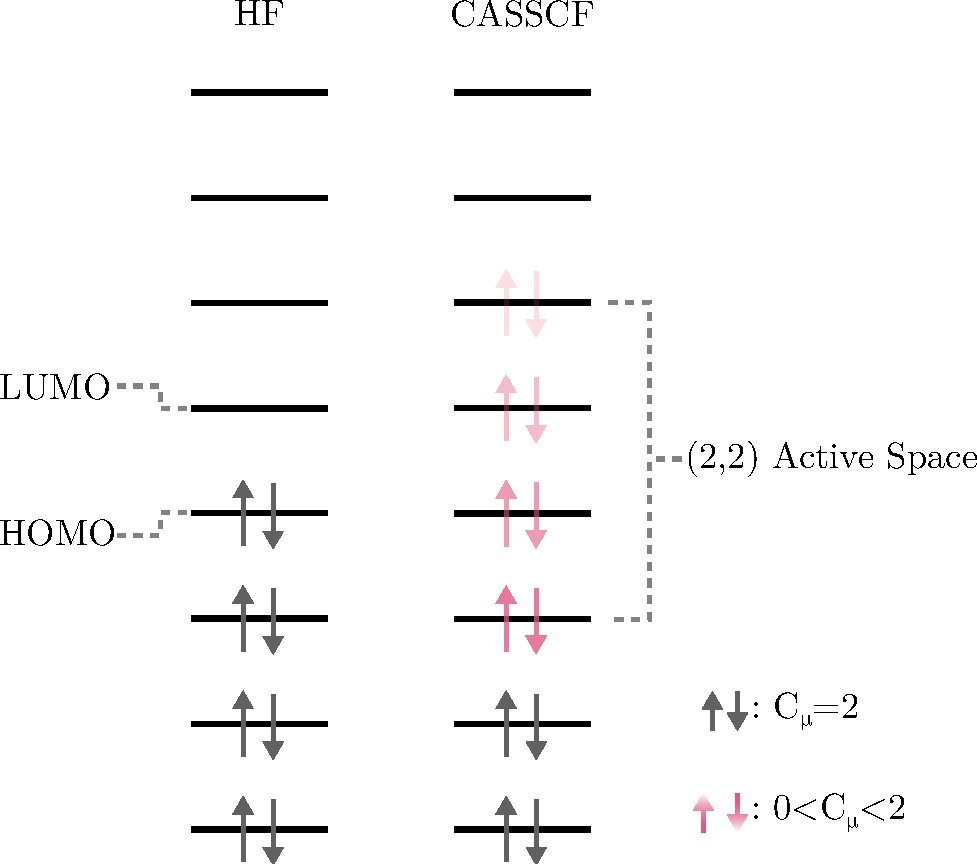
\includegraphics[width=10cm]{Chapters/2Methods/active_space.pdf}
\caption{Occupancy diagram of a closed shell Hartree-Fock wavefunction compared to a CASSCF(2,2) wavefunction. The occupancies $C_{\mu}$ are shown to be partial in the active space.}
\label{fig:cas}
\end{figure}

CASSCF recovers a large amount of correlation due to near-degenerate configurations, which are ignored in HF. However it does not encompass all of the low excitation determinants, as is for example done in CCSD. To correct for this type of correlation, we can apply a perturbative correction of second order to the multistate CASSCF wavefunction. This produces the Complete Active Space Perturbation Theory 2 method, CASPT2.\cite{Andersson1990,Andersson1992} Alternate implementations, such as CASMP2 where the correlation from an MP2 calculation is used, are also possible.\cite{McDouall1988}

\section{Density Functional Theory}

The previous section lists some of the most successful methods of calculating electronic properties of chemical systems by approximating their wavefunctions. However some of the most popular quantum chemistry methods today avoid calculating the wavefunction altogether, in favour of focusing on the electronic density as the principal state function.

\subsection{The Hohenberg-Kohn Theorems}
If we wish to express the energy of a system of $N$ interacting electrons under some external potential $v_{\text{ext}}$, we can write:
\begin{equation}
    E_{v_{\text{ext}}}[v_{\text{ext}},n] = \int n(\bm{r}) v_{\text{ext}}(\bm{r}) d\bm{r} + F[n]
\end{equation}
Where $n$ is the electron density and $F[n]$ is the \textit{universal functional} which maps $n$ to the energy of the enclosed $N$ interacting electron system.

Hohenberg and Kohn proved in the 1960s two fundamental theorems related to the electronic density $n$:\cite{Hohenberg1964}
 \begin{enumerate}
     \item The external potential of a quantum system $v_{\text{ext}}$ has a one-to-one correspondence with its electron density $n(\bm{r})$.
     \item The density which minimises the total energy of the system is the real ground state density.
 \end{enumerate}

Theorem 1 implies that the energy of the system is a functional of its electron density, $E_{v_{\text{ext}}}[v_{\text{ext}},n] \equiv E_{v_{\text{ext}}}[n]$. Theorem 2 states that we can find this density by evaluating its energy at each point, and varying it until we have found the minimum. This framework is known as Density Functional Theory (DFT). However, since the form of $F[n]$ is unknown, we must employ an approximation.

\subsection{Kohn-Sham theory}
The universal functional $F[n]$ is composed of the kinetic energy of the electron cloud $T[n]$ and the electron-electron interactions $W[n]$. The kinetic part is nontrivial to solve for electron densities, and the second one can be chosen to be the Coulomb interaction. In their wavefunction operator form, we would write:
\begin{equation}
    \hat{F}=\hat{T}+\hat{W}
\end{equation}

Where now the kinetic energy operator $\hat{T} = - \frac{\nabla^2}{2}$ is easy to solve for wavefunctions of a known form. We begin our model by imagining a set of $N$ non-interacting electrons submitted to a fictitious$v_s(\bm{r})$. We can write their secular equations as:\cite{Sham1965}
\begin{equation}
    (\hat{T} + v_s(\bm{r})) \varphi_i (\bm{r}) = (- \frac{\nabla^2}{2} + v_s(\bm{r})) \varphi_i (\bm{r}) = \epsilon_i \varphi_i (\bm{r})
    \label{eq:ks1}
\end{equation}
 
Where the eigenfunctions $\varphi_i (\bm{r})$ are known as the Kohn-Sham (KS) orbitals. The idea is to construct a KS wavefunction $\Psi_{\text{KS}}(\bm{x}_1,\ldots,\bm{x}_N)$ from the Slater determinant of the $N/2$ lowest energy spatial KS orbitals. For this to work, we need $v_s(\bm{r})$, which we call the KS potential, to accurately represent all of the electron-electron interactions which, based on the first Hohenberg-Kohn theorem, would yield a unique electron density:

\begin{equation}
n(\bm{r}) = \int |\Psi_{\text{KS}}(\bm{x}_1,\ldots,\bm{x}_{N/2})|^2 d\bm{x}_1\ldots d \bm{x}_{N/2} = 2\sum_j^{N/2} |\varphi_i(\bm{r})|^2
\label{eq:ks2}
\end{equation}

The second Hohenberg-Kohn theorem requires this density to minimise the total energy functional. Fortunately, there is a systematic way of improving the accuracy of the wavefunction, and thus variationally reducing its energy. The external potential $v_s(\bm{r})$ must depend on the solutions of Equation \ref{eq:ks1}. This means that they can be solved iteratively, in an SCF procedure analogous to that of HF. Equations \ref{eq:ks1} and \ref{eq:ks2} are known as the KS equations, and form the basis of KS DFT.

\subsection{The Kohn-Sham Potential}

We have yet to comment on the form of $v_s(\bm{r})$. Since it depends on the density, we write it as a functional:
\begin{equation}
    v_s[n](\bm{r}) = v_{\text{ext}}(\bm{r}) + v_{\text{Har}}[n](\bm{r}) + v_{\text{XC}}[n](\bm{r})
    \label{eq:external}
\end{equation}

Where the first term is the external potential, including nuclear potentials under the BO approximation but also any external imposed potentials $v_{\text{field}}(\bm{r})$ to the system:
\begin{equation}
    v_{\text{ext}}(\bm{r}) = v_{\text{field}}(\bm{r}) + \sum_i^{N_Z} \frac{Z_i}{|\bm{R}_i - \bm{r}|}
    \label{eq:ext_decomp}
\end{equation}
Where we have considered $N_Z$ nuclei at positions $\bm{R}_i$ with charge $Z_i$.

The second term of Equation \ref{eq:external} is the Hartree potential:
\begin{equation}
    v_{\text{Har}}[n](\bm{r}) = \int \frac{n({\bm{r}')}}{|\bm{r} - \bm{r}'|}d\bm{r}'
\end{equation}
Which represents the electron-electron Coulomb potential.

The final term of Equation \ref{eq:external} should represent all other electron-electron interactions, namely exchange and correlation. We write it as the derivative of the exchange-correlation functional $E_{\text{XC}}[n]$:
\begin{equation}
    v_{\text{XC}}[n](\bm{r}) = \frac{\delta E_{\text{XC}}[n]}{\delta n(\bm{r})}
\end{equation}
We write it in this form because we will need the exchange-correlation functional when calculating the energy of the KS DFT system.

\subsection{The Exchange-Correlation Functional}

$E_{\text{XC}}[n]$ does not have a known exact solution, and we therefore adopt certain approximations in order to carry out DFT calculations.

\subsubsection{Local Density Approximation}
The simplest non-trivial exchange-correlation functional uses the analytical solution for the exchange energy density of a homogeneous electron gas $e^h_{\text{x}}(n(\bm{r}))$. The correlation part of the energy, $e^h_{\text{c}}(n(\bm{r}))$, has no known solution but one can parameterise it to match those of very accurate quantum Monte Carlo calculations.\cite{Tanatar1989}

We can write the functional as the integral of the two energy densities:
\begin{equation}
    E^{\text{LDA}}_{\text{XC}}[n] = \int e^h_{\text{x}}(n(\bm{r})) + e^h_{\text{c}}(n(\bm{r})) d\bm{r}
\end{equation}

This functional is named the Local Density Approximation (LDA), since at each point, it only conveys the non-Coulombic many-electron interactions of an uniform electron gas with the density of the point. Surprisingly, this approximation still recovers the correct general structure of many bulk solids, for instance, though the error in energy is in the range of 1 eV per atom, which renders it poorly suited to quantitative prediction.\cite{Zhang2018}

\subsubsection{Generalised Gradient Approximation}
LDA functionals can be improved by using the exchange and correlation from the fictitious system of the electron gas of constant gradient, instead of constant density. In the general terms, these Generalised Gradient Approximation (GGA) functionals can be written:
\begin{equation}
    E^{\text{GGA}}_{\text{XC}}[n(\bm{r})] = \int e^{\text{GGA}}_{\text{XC}}(n(\bm{r},\nabla n(\bm{r})) d\bm{r}
\end{equation}

The GGA exchange-correlation energy density $e^{\text{GGA}}_{\text{XC}}$ can take many forms. For example, one of the most popular GGA functionals, developed by Perdew, Becke and Ernzerhof\cite{Perdew1996} (PBE), was developed in order to be completely \textit{ab intio} and satisfies as many exact properties of the KS wavefunction as possible. For instance, it is favoured by the community which simulates metal-organic frameworks for its affordability\textemdash{}given unit cells of up to hunders of atoms\textemdash{}and accuracy in modelling bond angles with a precision greater than 0.1 \AA{}.\cite{Nazarian2015}

One could also list the Becke 1988 exchange functional, B88\cite{A.D.Becke1988}, or the Lee-Yang-Parr correlation functional (LYP)\cite{Lee1989} which combine into the BLYP functional.

\subsubsection{Hybrids}
A further improvement to consider is that of including exchange from a wavefunction-based calculation into our results. Indeed HF calculations have no correlation by definition but provide exact nonlocal exchange:
\begin{equation}
    e^{\text{exact}}_{\text{x}} = - \frac{1}{2} \sum_{\sigma} \sum_{i,j=1}^{N_{\sigma}}
    \frac{
    \varphi^*_{i \sigma}(\bm{r}') \varphi_{j \sigma}(\bm{r}')
    \varphi_{\sigma i}(\bm{r}') \varphi^*_{j \sigma}(\bm{r}') 
    d\bm{r}'
    }{
    |\bm{r} - \bm{r}'|
    }
\end{equation}
Where the $\sigma$ indices represent spin up or down.

By mixing this exact exchange with different proportions of LDA and GGA terms, one can construct hybrid exchange-correlation functionals. PBE0 combines PBE with exact exchange\cite{Adamo1999} for increased accuracy. The Heyd–Scuseria–Ernzerhof (HSE) functional screens the exchange part of PBE0 with an error function for added efficiency, calculating the long-range exchange with PBE.\cite{Heyd2003,Heyd2006} B3LYP is a three parameter exchange-correlation functional which mixes LDA and B88 exchange with LDA and LYP correlation.\cite{Stephens1994} B3LYP is currently the most used density functional\cite{Zhang2010}, and predicts bond lengths of bulk TiO$_2$ with an accuracy of 0.01\AA{}, compared to 0.1 \AA{} for LDA.

\subsubsection{Range Separated Hybrids}
Other combinations of exchange and correlation terms are possible, and they can be screened by a distance parameter, in order to assign short-range energies to the best performing short-range functionals and \textit{vice versa} for long-range ones. Here, we will only mention $\omega$B97X-D,\cite{Chai2008} which uses the Becke 97 short-range GGA functional\cite{Becke1997} and combines it with long-range HF exchange and a small portion of short-range H exchange. It reproduced CC2 excitation energies with a 0.2 eV accuracy on biochromophores, indicating a high reliability.\cite{Shao2020}

The long-range behaviour of exchange-correlation interactions is particularly relevant to intermolecular processes, since the interactions between monomers is beyond the distance of atomic bonds. In particular, excited state wavefunctions are typically more diffuse than their corresponding ground state, further justifying the use of range-separated functionals. Important delocalised phenomena such as charge transfer require such tools.


\subsubsection{Dispersion Correction}
Due to the parameterisation of the correlation functional at the root of LDA theory, KS DFT often omits the long-range correlation between electrons which results in dispersion (sometimes called van der Waals interaction), even when mixing HF exchange.

Grimme's D2 method\cite{Grimme2006} accounts for the dispersion of the system \textit{a posteriori}, allowing for the correction of any of the functionals described above. In fact the \textit{D} in $\omega$B97X-D implies that this functional already uses Grimme's D2 correction.

\subsection{Density Functional Tight-Binding}

DFT is also the basis of a variety of semi-empirical methods, which aim to combine the efficiency of classical simulation with the accuracy of an electronic description. Prominently, the Density Functional Tight-Binding (DFTB) model eschews the determination of a KS density. Instead, it uses atomic KS orbitals, which have been previously parameterised through DFT calculations. The atomic orbitals are then combined in a Taylor expansion of the exchange-correlation functional.\cite{Foulkes1989,Seifert2012}

The order of this Taylor expansion ranges in practice from one to three, where the first order energy expression is:
\begin{equation}
    E^{\text{DFTB1}}=\sum_{i}n_i \epsilon_i + \frac{1}{2}V^{\text{rep}}_{ab}
\end{equation}

Where $n_i$ is the occupation of KS orbital $i$, $\epsilon_i$ is its orbital energy, and $V^{\text{rep}}_{ab}$ are repulsive pair potentials either fitted from DFT calculations or from empirical data.\cite{Elstner1998}

For organic systems, routine calculations usually use the second order, where density fluctuations are considered for all atoms. In this case, the atomic charge density fluctuations are modelled as exponentially decaying distributions with a decay parameter $\tau_a$ fitted to DFT calculations:
\begin{equation}
    \delta \rho_a(\bm{r}) \approx \Delta q_a \frac{\tau_a^3}{8\pi}e^{-\tau_a\abs{\bm{r}-\bm{R}_a}}
\end{equation}
Where $\Delta q_a$ is the fluctuation in partial charge on a given atom $a$, and $\bm{R}_a$ is the position of the atomic nucleus.

The energy becomes:
\begin{equation}
    E^{\text{DFTB2}}=E^{\text{DFTB1}} + \frac{1}{2}\sum_{ab} \Delta q_a \Delta q_b \gamma_{ab}(\tau_a,\tau_b,R_{ab})\end{equation}

 Where $\gamma_{ij}(\tau_i,\tau_j,R_{ij})$ is an analytical function resulting from evaluating the Hartree energy between the decaying charge densities and $R_{ij}$ is the distance between two atomic centres.\cite{Foulkes1989}
 
 Second order DFTB can be very accurate when applied to well-studied systems, since it is semi-empirical. Indeed it matches the accuracy of B3LYP in calculating geometrical parameters of TiO2 nanostructures.\cite{Selli2017}
\section{Solid State Electronic Structure}

Not only has DFT found success in molecular systems, it has also been formulated to address problems in systems with a natural periodicity such as crystals, surfaces or polymers.

\subsection{The Periodic Lattice}



The defining feature of a crystal is that its structure has a given periodicity. We call the smallest repeating unit constituting the whole crystal by translations the \textit{unit cell}. These translations determine the shape of the unit cell, and we therefore usually define a unit cell by it's three primitive lattice vectors $\bm{a}_1$, $\bm{a}_2$, and $\bm{a}_3$.

Any atom within the unit cell is therefore located at:
\begin{equation}
    \bm{R}_s = s_1\bm{a}_1 + s_2\bm{a}_2 + s_3\bm{a}_3
\end{equation}
Where $0\le{}s_i<1$. By definition, given an arbitrary number of transitions $n_1$, $n_2$ and $n_3$ such that $n_i \in \mathbb{Z}$, there are atoms of the same type at all positions:
\begin{equation}
    \bm{R}' = \bm{R} + n_1\bm{a}_1 + n_2\bm{a}_2 + n_3\bm{a}_3 \equiv \bm{R} + \bm{L_{n_1,n_2,n_3}}
\end{equation}
Where we have defined $\bm{L_{n_1,n_2,n_3}}$ as an arbitrary lattice translation. By this process, an entire lattice can be constructed as shown in Figure \ref{fig:lat_diag}.

\begin{figure}
\centering
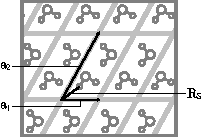
\includegraphics[width=7cm]{Chapters/2Methods/lattice_diagram.pdf}
\caption{Schematic representation of the role of the unit cell in generating a lattice. In this 2-D example, $\bm{a}_1$ and $\bm{a}_2$ are lattice vectors, and $\bm{R}_s$ is an atomic position in the unit cell.}
\label{fig:lat_diag}
\end{figure}

\subsection{Bloch's Theorem}
We now wish to describe the wavefunction of electrons in a periodic array of nuclei, which is the application of the BO approximation to the crystal. The Schr\"{o}dinger equation is in this case:
\begin{equation}
    \left( - \frac{\nabla^2}{2} + V(\bm{r})\right) \psi(\bm{r}) = E\psi(\bm{r})
\end{equation}
Where the periodic potential is $V(\bm{r}) = V(\bm{r} + \bm{L_{n_1,n_2,n_3}})$ for any lattice translation.

It can be shown that electrons in periodic potentials have wavefunctions in a basis of the form:
\begin{equation}
    \psi_{n\bm{k}}(\bm{r}) = e^{i\bm{k}\cdot\bm{r}} u_{n\bm{k}}(\bm{r})
    \label{eq:bloch}
\end{equation}

Where $n$ is the integer energy level of the wavefunction, $\bm{k}$ is called the \textit{crystal wave vector} and has a dimension of inverse distance, and $u_{n\bm{k}}(\bm{r})$ is a function with the periodicity of the potential. These basis functions are called \textit{Bloch waves}.


\subsection{Reciprocal Space}

We now examine what would happen to the Bloch wave if $\bm{k}$ is shifted by any vector $\bm{b}_n$ such that $\bm{b}_i\cdot\bm{a}_j=2\pi\delta_{ij}$, where the set of $\bm{a}_n$ vectors defines the periodicity of the potential.

\begin{equation}
    \begin{split}
        \psi_{n(\bm{k}+\bm{b})}(\bm{r}) &= e^{i(\bm{k}+\bm{b})\cdot\bm{r}} u_{n(\bm{k}+\bm{b})}(\bm{r})\\
        &= e^{i\bm{k}\cdot\bm{r}} e^{i\bm{b}\cdot\bm{r}} u_{n(\bm{k}+\bm{b})}(\bm{r})\\
        &= e^{i\bm{k}\cdot\bm{r}} \tilde{u}_{n(\bm{k}+\bm{b})}(\bm{r})
    \end{split}
\end{equation}

For the cases where $\bm{r}' = \bm{L_{n_1,n_2,n_3}}$, we have $e^{i\bm{b}\cdot\bm{r}'}=e^{i2n\pi}=1$, which means that the function $\tilde{u}_{n(\bm{k}+\bm{b})}(\bm{r}) = e^{i\bm{b}\cdot\bm{r}} u_{n(\bm{k}+\bm{b})}(\bm{r})$ has the same periodicity as $V(\bm{r})$. $\psi_{n(\bm{k}+\bm{b})}(\bm{r})$ can therefore be expressed as a Bloch wave with wave number $\bm{k}$, and presuming non-degenerate Bloch states, $\tilde{u}_{n(\bm{k}+\bm{b})}(\bm{r}) = u_{n\bm{k}}(\bm{r})$ and $\psi_{n(\bm{k})}(\bm{r}) = \psi_{n(\bm{k}+\bm{b})}(\bm{r})$. This result can also be shown to hold for degenerate Bloch states. In other words, $\bm{k}$ is periodic with respect to the vectors $\bm{b}_n$.

We call the inverse distance space of the lattice \textit{reciprocal space}. It follows that the vectors $\bm{b}_n$ are reciprocal primitive lattice vectors which form a space analogous to the primitive cell called the \text{1st Brillouin Zone} (1BZ).

\subsection{k-point Sampling}
We have observed that electronic wavefunctions in crystals are expressed in the basis of Bloch waves. Therefore, setting aside the calculation of $u_{n\bm{k}}(\bm{r})$, the representation of the wavefunction can be improved by increasing the size its basis, and therefore considering Bloch waves of more $\bm{k}$ values. The cost of a periodic DFT calculation is multiplied for each k-point considered, so it is important to calculate as few as necessary to represent the required properties of the system.

k-points can be understood as representing the periodicity of the material, therefore unit cells with a small lattice vector $\bm{a}_1$ should have a large amount of k-points in the $\bm{b}_1$ direction, and \textit{vice versa}. In practice, we often use a grid of $N_1$x$N_2$x$N_3$ k-points, where the $N_i$ values are chosen to be approximately inversely proportional to the lengths of the lattice vectors $\bm{a}_1$, $\bm{a}_2$, and $\bm{a}_3$. This defines the Monkhorst-Pack grid.\cite{Monkhorst1976}

\subsection{Plane Wave Basis Sets}
We now wish to calculate the $u_{n\bm{k}}(\bm{r})$ term of Equation \ref{eq:bloch} using DFT. As in the case of molecular systems, periodic systems need to be decomposed in a basis in order to calculate the matrix elements of the external potential.

Since the wavefunction is periodic, its basis functions must also have a periodicity. We choose to use plane waves because their periodicity is easily tunable and their products can be integrated very efficiently using fast Fourier transforms.

\begin{equation}
    u_{n\bm{k}}(\bm{r}) = \sum_{\bm{G}} c_{\bm{G},\bm{k}} e^{i\bm{G}\cdot \bm{r}}
\end{equation}

Where $\bm{G}$ are reciprocal lattice vectors. As $|\bm{G}|$ becomes larger, the expansion coefficients $c_{\bm{G},\bm{k}}$ become smaller and therefore these terms of the expansion less important. Since we need to select a finite number of $\bm{G}$ values for computation, we choose a cut-off value $G_{\text{cut}}$ such that we only include plane waves with $|\bm{G}| \leq G_{\text{cut}}$ in the expansion.

This method works well for valence electrons, however since the energies of the electrons nearest to the nuclei are comparatively very high, we would need basis functions of a higher frequency to represent them and therefore a very high $G_{\text{cut}}$. To avoid this, we usually avoid representing core electrons altogether, since they are unlikely to be involved in the chemical processes we are interested in. Instead, we represent the combined effect of the nucleus and the core electron's screening by functions called \textit{pseudopotentials}.

\subsection{The Ewald Potential}
\label{sec:ewald}
This subsection is adapted from \textit{ONIOM(QM:QM') Electrostatic Embedding Schemes for Photochemistry in Molecular Crystals} by Miguel Rivera, Michael Dommett, and Rachel Crespo-Otero.\cite{Rivera2019}

An additional subtlety of performing DFT calculations in periodic systems comes from the new form of the nuclear potential. Indeed, the external potential of the KS equations has a component which is traditionally composed of atom centred point charges of the value of the atomic number. This is the second term in Equation \ref{eq:ext_decomp}. However in a periodic system, there are infinite nuclei involved, and the potential is therefore impossible to compute through direct summation.

A na\"{i}ve approach would be to choose a large spherical region of the crystal, and, for each KS equation, consider only the nuclei of the crystal that fall within the chosen radius. Unfortunately, the Madelung sum\textemdash{}the electrostatic potential of the whole lattice\textemdash{}is known to be a slowly and conditionally convergent property.\cite{Kittel1986,Kantorovich2004} The former is due to the fact that Coulomb decay as an inverse law with distance, which is much further reaching than other forms of interatomic interactions like exchange. The latter can be understood from the fact that lattice has discrete sites in space which are not equally spaced from a particular point. Thus a radial truncation will necessarily be imbalanced towards some directions more than others.

The long-range Coulomb interactions with distant atomic centres are therefore traditionally evaluated using the Ewald summation technique\cite{Weber2010,Torras2008,McKenna2007}. The expression for the Ewald potential at position $r$ is:

\begin{equation}
V^{\text{Ewald}} ( \bm{r} ) = \sum_{\bm{L}s} q_s \frac{\erfc{}(\gamma|\bm{r} - \bm{L} - \bm{R}_s|)} {|\bm{r} - \bm{L} - \bm{R}_s|}
+ \frac{4 \pi} {v_c}
\sum_{\bf{G}\neq 0} \frac{1}{G^2} e^{-G^2/4\gamma^2}
\Bigg{[}\sum_s q_s e^{i\bm{G}(\bm{r} - \bm{R}_s )}\Bigg{]}
\label{eq:ewald}
\end{equation}
Where $\bm{L}$ and $\bm{G}$ are the real and reciprocal space lattice translations, $q_s$ are the charges of each site $s$ of the unit cell at positions $\bm{R}_s$, $\gamma$ is the Ewald constant and $v_c$  is the volume of the unit cell. Here, the direct sum electrostatic potential has been recast as a sum of two rapidly converging series. Short-range Coulomb terms are calculated in direct space and long-range interactions using a Fourier series in reciprocal space. To evaluate the Ewald potential on a lattice site $\bm{R}_i$, the self-potential of the charge must be subtracted to avoid a singularity which amounts to replacing the $\bm{L} = 0$ and $s = i$ case of the first term of Equation \ref{eq:ewald} with $- \frac{2 \gamma q_i}{\sqrt{\pi}}$.\cite{Kantorovich2004,Kittel1986,Toukmaji1996,Sauer1989a}


\section{Excited States}
\label{sec:excited}
The methods outlined above focused on obtaining accurate and affordable ground state properties of chemical systems. However many processes of practical interest involve excited state systems which require specialised methods to model. We will first show how to extend DFT to the excited state and then focus on wavefunction based methods.

\subsection{Linear-Response}

We wish to obtain observable quantities, such as the density, from an optically excited system. This can be understood as investigating a system which starts in the ground state and is perturbed by a time-dependent potential $v(\bm{r},t)$ infinitesimally later than a time $t_0$, where this potential will have the same frequency as the incident photon.

The difference in density between a time $t$ and the initial perturbation time $t_0$ is called the \textit{response} of the density ($n(t)-n(t_0)$). This response can be expanded in powers of $v(\bm{r},t)$:
\begin{equation}
    n(t)-n(t_0) = n_1(t) + n_2(t) + \ldots
\end{equation}

The first and largest term of this expansion is called the \textit{linear response} of the density. It is written:
\begin{equation}
    n_1(\bm{r},t) = \int^{\infty}_{0} dt' \int d\bm{r}  \chi_{nn}(\bm{r},\bm{r}',t-t') v_1(\bm{r},t)
\end{equation}

Where $v_1(\bm{r},t)$ is the linearised time-dependent potential and $\chi_{nn}(\bm{r},\bm{r}',t-t')$ is the density-density response function defined as:
\begin{equation}
    \chi_{nn}(\bm{r},\bm{r}',t-t') = -i\theta(t-t')\bra{\Psi_0}[\hat{n}(\bm{r'},t-t'),\hat{n}(\bm{r})]\ket{\Psi_0}
\end{equation}

Where we have introduced the density operator $\hat{n}(\bm{r}) = \sum_i \delta(\bm{r}-\bm{r}_i)$ where the summation is over all electrons.

This expression can be recast into the frequency domain and shown to depend on the excitation energies of the system $\Omega_n = E_n - E_0$ where the energies are associated with the excited state wavefunctions $\Psi_n$:
\begin{equation}
    \chi_{nn}(\bm{r},\bm{r}',\omega) = \lim_{\eta\to+0} \sum^{\infty}_{n=1} \left\{ 
    \frac{\bra{\Psi_0}\hat{n}(\bm{r})\ket{\Psi_n} \bra{\Psi_n}\hat{n}(\bm{r}')\ket{\Psi_0}}{\omega - \Omega_n + i\eta}
    -
    \frac{\bra{\Psi_0}\hat{n}(\bm{r}')\ket{\Psi_n} \bra{\Psi_n}\hat{n}(\bm{r})\ket{\Psi_0}}{\omega + \Omega_n + i\eta}
    \right\}
    \label{eq:lehmann}
\end{equation}


Where $\omega$ is the frequency of the perturbation, and $\eta$ is a vanishingly small positive scalar chosen to avoid unphysical infinite response values. This is known as the Lehmann representation, and shows that if we can obtain an expression for $\chi_{nn}(\bm{r},\bm{r}',\omega)$, we know that its poles will yield the excitation energies of the system.

\subsection{Time-Dependent Density Functional Theory}

We wish to use some of the pre-established formalisms of DFT in our efforts to define a DFT density-density response function, hopefully culminating in a time-dependent DFT (TDDFT). We begin with the fundamental theorem of TDDFT:

\begin{itemize}
    \item The time-dependent external potential of a quantum system $v(\bm{r},t)$ has a one-to-one correspondence with its time-dependent electron density $n(\bm{r},t)$ up to a time-dependent phase.
\end{itemize}
This is known as the Runge-Gross theorem and it ensures that the correspondence established before $t_0$ by the first Hohenberg-Kohn theorem is maintained during the perturbation of the system. The second theorem can be cast into the time-dependent case by showing that the time-dependent density determines the action of the quantum system, which itself should be minimised by the variational theorem for the real wavefunction.

\subsection{The Kohn-Sham Response Function}
We are therefore justified in taking the steps of calculating the density-density response function in the non-interacting KS system. The principal difference will be that the linearised external potential has the form:
\begin{equation}
    v_{s1} = v_1(\bm{r},t) + \int \frac{n_1(\bm{r},t)}{|\bm{r}-\bm{r}|}d\bm{r} + v_{\text{xc}1}(\bm{r},t)
\end{equation}

Where the first term is the linearised perturbation potential, the second is the Hartree potential, and the third the linearised exchange-correlation potential:
\begin{equation}
    v_{\text{xc}1}(\bm{r},t) = \iint \frac{\delta v_{\text{xc}}[n](\bm{r},t)}{\delta n(\bm{r',t})} \Bigr|_{n(\bm{r},t_0)} n_1(\bm{r},t') d\bm{r} dt'
\end{equation}

Where we use the shorthand:
\begin{equation}
    f_{\text{xc}} (\bm{r},t,\bm{r}',t') =\frac{\delta v_{\text{xc}}[n](\bm{r},t)}{\delta n(\bm{r',t})} \Bigr|_{n(\bm{r},t_0)}
\end{equation}

This is called the exchange-correlation kernel and is analogous to the exchange-correlation functional in ground state DFT, where the same approximations can be employed. In practice, the time dependence of this kernel implies that it depends on all past fluctuations of the density. An approximation to circumvent this tremendous requirement is to fix the kernel to its value at the beginning of the perturbation. This constitutes the \textit{adiabatic local density approximation}. 

A further improvement is to cast the kernel into the frequency domain, then written $ f_{\text{xc}}(\bm{r},\bm{r}',\omega)$, simplifying our task by using the periodicity of the perturbation. This is called the frequency dependent LDA.

Still in the frequency domain, we can construct a KS linear response of the density by means of a Fourier transform:
\begin{equation}
    n_1(\bm{r},\omega) = \int \chi_s(\bm{r},\bm{r'},\omega) \left[v_1(\bm{r}',\omega) + \int \left(\frac{1}{|\bm{r}'-\bm{x}|} + f_{\text{xc}}(\bm{r}',\bm{x},\omega) \right) n_1(\bm{x},\omega)d\bm{x}\right] d\bm{r}'
\end{equation}

Where the KS density-density response function is:
\begin{equation}
    \chi_s(\bm{r},\bm{r'},\omega) = \sum_{j,k=1}^{\infty} (f_k - f_j)
    \frac{\varphi^0_j(\bm{r})\varphi^{0*}_k(\bm{r})\varphi^{0*}_j(\bm{r}')\varphi^0_k(\bm{r}')}
    {\omega-\omega_{jk}+i\eta}
\end{equation}

Where $f_j$ and $f_k$ are the occupancies of the KS orbitals at time $t_0$, $\varphi^0_j$ and $\varphi^0_k$, in the ground state and $\omega_{ij}=\epsilon_j - \epsilon_k$ where $\epsilon_j$ and $\epsilon_k$ are the orbital energies. Ideally, the KS original excitation energies $\omega_{ij}$ should match the real excitations $\Omega_n$ of Equation \ref{eq:lehmann}, relying upon the fact that the KS orbital transitions form a sufficient basis to represent this excitation. This hinges upon the form of the exchange-correlation functional, which explains its importance.

\subsection{The Casida Formulation}
We would like to formulate the above linear response problem into an eigenproblem, which is solvable in a direct way.

We first construct a coupling-matrix for the KS orbital transitions and add a spin index to each KS orbital:
\begin{equation}
    K_{jk\sigma,j'k'\sigma'} = \iint \varphi^{0*}_{j\sigma}(\bm{r})\varphi^0_{k\sigma}(\bm{r})
    \left(\frac{1}{|\bm{r} -\bm{r}'|} + f_{\text{xc}}(\bm{r},\bm{r}',\Omega) \right)
    \varphi^{0*}_{j'\sigma'}(\bm{r}')\varphi^0_{k'\sigma'}(\bm{r}')
    d\bm{r}' d\bm{r}
\end{equation}

We can write the tensors:
\begin{equation}
    \begin{split}
        A_{ia\sigma,i'a'\sigma'}(\Omega) &= \delta_{ii'}\delta_{aa'}\delta_{\sigma\sigma'}\omega_{a'i'\sigma'} + K_{ia\sigma,i'a'\sigma'}(\Omega)\\
        B_{ia\sigma,i'a'\sigma'}(\Omega) &= K_{ia\sigma,i'a'\sigma'}(\Omega)
    \end{split}
\end{equation}

Each element of the $A_{ia\sigma,i'a'\sigma'}(\Omega)$ and $B_{ia\sigma,i'a'\sigma'}(\Omega)$ tensors represents an individual KS orbital transition. We can build an anti-Hermitian eigenvalue problem which will tell us the contributions from each of these transitions to a given excitation:
\begin{gather}
    \begin{pmatrix}
    \mathbb{A}&\mathbb{B}\\
    \mathbb{B}&\mathbb{A}
    \end{pmatrix}
    \begin{pmatrix}
    \bm{X}\\
    \bm{Y}
    \end{pmatrix}
    =
    \Omega
    \begin{pmatrix}
     - \mathbb{1}&0\\
    0&\mathbb{1}
    \end{pmatrix} 
    \begin{pmatrix}
    \bm{X}\\
    \bm{Y}
    \end{pmatrix}
\end{gather}

Where the elements of $\bm{X}$ and $\bm{Y}$ can be shown to correspond to the orbital transition coefficients for the single excitation of energy $\Omega$. These are called the Casida equations,\cite{Casida1998} and they enable us to efficiently calculate excitation energies, occupancies and oscillator strengths of excited states in TDDFT.


\subsection{Algebraic Diagrammatic Construction}
We aim to produce an excited state wavefunction of N electrons without using the density as the state function, which defines DFT. To do so, we first calculate all of the states resulting from the single excitations of a ground state wavefunction. Since they are not, in general, orthonormal, we employ successive Gram-Schmidt orthogonalisations to build a satisfactory basis of intermediate states $\{\ket{\tilde{\Psi}^N_J}\}$.\cite{Schirmer2004}

We now build the so-called Algebraic Diagrammatic Construction (ADC) matrix:
\begin{equation}
    M_{IJ}=\bra{\tilde{\Psi}^N_I}\hat{H}-E^N_0\ket{\tilde{\Psi}^N_J}
\end{equation}

Where we have shifted the Hamiltonian by the ground state energy $E^N_0$. This matrix yields the eigenvalue equation:
\begin{equation}
    \bm{MX}=\bm{X\Omega}
\end{equation}
Where $\bm{\Omega}$ is the diagonal matrix of eigenvalue excitation energies $\Omega_n$ and $\bm{X}$ has values used to reconstruct the exact wavefunction from the basis of intermediate states like so:
\begin{equation}
    \ket{\Psi^N_n} = \sum_J X_{nJ} \ket{\tilde{\Psi}^N_J}
\end{equation}

To carry out this scheme, we need an accurate ground state wavefunction. A common choice is the MP2 wavefunction, which yields the ADC2 excited state wavefunction.\cite{Trofimov1995,Trofimov1997}

\subsection{Excited State Coupled Cluster}

CC methods can also be cast into an eigenvalue form for the excited states:\cite{Sneskov2012}
\begin{equation}
    \bm{AR}=\bm{\Omega{}R}
\end{equation}
Where the $\bm{A}$ matrix arises from linear response theory, much in the same spirit of Casida TDDFT:
\begin{equation}
    A_{\mu_i \nu_j} = \bra{\mu_i} e^{-\hat{T}}[\hat{H},\hat{\tau}_{\mu_j}]\ket{\Psi^0_{\text{CC}}}
\end{equation}

Where $\hat{\tau}_{\mu_j}$ is the $i$-tuple excitation operator and $\mu_i$ the collection of orbitals involved in this excitation.

In this paradigm, one can employ the full CCSD expression for the ground state, and only use perturbative double excitations for the excited state. The resulting scheme is called CC2 and scales with a power of $N^5$ orbitals instead of the $N^6$ of CCSD.\cite{Christiansen1995}

\subsection{Multireference Methods (bis)}

Finally, multireference methods can also naturally be applied to the excited state, as can be understood from Section \ref{sec:multiref}. CASSCF excited state calculations are usually calculated in a state-averaged way, in order to take into account the different excited states in the total density.

CASPT2 can apply its dynamic correlation correction to several state-averaged CASSCF wavefunctions simultaneously.\cite{Almlof1981} This is called Multistate CASPT2 or MS-$N$-CASPT2 where $N$ is the amount of excited states.\cite{Finley1998} It is a method of state-of-the-art accuracy, for example predicting a vertical singlet excitation of 7.98 eV in ethene, compared to the best estimate of 7.8 eV, where CC2 predicts 8.40 eV.\cite{Schreiber2008}

Multireference methods are necessary to model highly nonadiabatic regions of the PES, such as bond breaking or conical intersections, which are discussed in Section \ref{sec:conicals_sec}. While ADC(2) and CC2 methods may be able to approximate the topology of certain conical intersections,\cite{Tuna2015} their pertinence is unpredictable, and CASSCF or CASPT2 are the most robust tools available for this task. In particular, TDDFT, a workhorse of excited state modelling, displays serious qualitative deficiencies in this domain.\cite{Levine2007}

Whilst the accounts of the accuracy of multireference methods for excited states are extensive,\cite{Silva-Junior2008,Silva-Junior2010,Helmich-Paris2019} their formidable cost limits their use. Indeed whilst most single reference methods discussed herein scale their cost with power laws, multireference methods scale factorially.\cite{Helmich-Paris2019a} This imposes significant restrictions to the system sizes and basis sets available to multireference methods. In particular, until recently, CASPT2 energy gradients could only be computed numerically,\cite{Shiozaki2018} making geometry optimisation out of the capabilities of routine calculations on institutional clusters for practically sized molecules.